\documentclass[12pt]{article}
\usepackage{amsmath}
\usepackage{amssymb}
\usepackage{graphicx}
\usepackage{color}
%\input labelfig.tex
\setlength{\parindent}{0pt} \oddsidemargin 0.0in \evensidemargin
0.0in \topmargin -1in \textheight 9.9in \textwidth 6.9in
\renewcommand{\baselinestretch}{1.02}
\usepackage{amsfonts,verbatim}
\usepackage{sectsty}
\sectionfont{\huge}
\subsectionfont{\Large}
\subsubsectionfont{\large}

\newcounter{question}[section]

\newenvironment{question}{\refstepcounter{question}\textbf{Question~\thequestion.}}{\bigskip}

\begin{document}

{\Large {\sf Math 158 - Homework 1}}

\bigskip


\begin{question}  Let $K_{n:r}$ denote the {\em Kneser graph}, whose vertex set is the
set of $r$-element subsets of an $n$-element sets, and where two vertices form an edge if the
corresponding sets are disjoint.
\begin{center}
\begin{tabular}{lp{5.5in}}
(a) & Describe $K_{n:1}$ for $n \geq 1$. \\
(b) & Draw $K_{4:2}$ and $K_{5:2}$. \\
(c) & Determine $|E(K_{n:r})|$ for $n \geq 2r \geq 1$.
\end{tabular}
\end{center}
\end{question}

\begin{enumerate}
    \item $V(K_{n:1})$ consists of all subsets of size 1 of [n],
    and all of these subsets are disjoint,
    so $K_{n:1}$ is isomorphic to the complete graph, $K_n$.
    \item To the left is $K_{4:2}$ and to the right is $K_{5:2}$.

    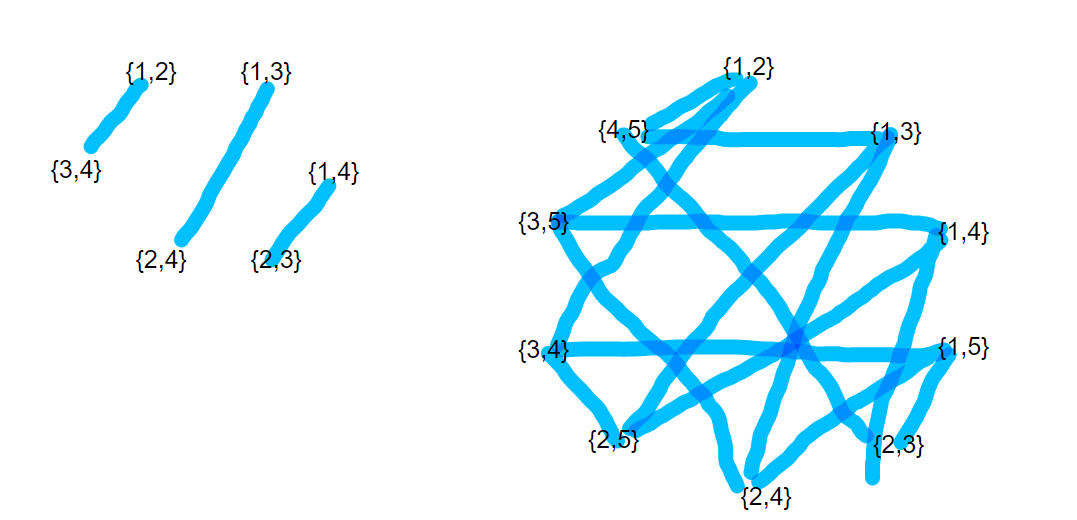
\includegraphics{CompleteGraphs.png}
    \item There are $\binom{n}{r}$ subsets and $\binom{n-r}{r}$
    subsets that are disjoint with any given subset.
    Thus the sum of the degrees of $K_{n:r}$ is $\binom{n}{r}\binom{n-r}{r}$,
    and so there are $\frac{1}{2}\binom{n}{r}\binom{n-r}{r}$ edges.
\end{enumerate}

\newpage

\begin{question}
Let $G$ be a digraph such that every vertex has positive in-degree. Prove that $G$ contains a directed cycle.
\end{question}

Let P be a directed path from $v_1$ to $v_r$.
Since every vertex has positive in-degree,
there must always be a vertex, $v_i$, that connects to $v_1$.
If $v_i$ is on the path, then G contains the cycle, $v_1v_2\hdots v_iv_1$.
If $v_i$ is not on the path, then adding $v_i$ to the path results in a longer path.
Since G contains a finite number of vertices, repeatedly adding vertices
to the path will eventually result in a cycle.
\newpage


\begin{question}     Let $G$ be an $n$-vertex graph with $n \geq 2$ and
$\delta(G) \geq (n - 1)/2$. Prove that $G$ is connected and that the diameter of
$G$ is at most two.
\end{question}

Picking two arbitrary vertices, $v, w$, as the ends of a path.
The neighborhoods of both vertices must overlap by the pigeonhole principle.
There are $n-2$ verticies that are not $v$ or $w$, yet each end of the path
must be adjacent to at least $\frac{n-1}{2}$ other vertices.
Thus $v$ and $w$ must either be directly adjacent to each other,
or they must share a neighbor with which they are both adjacent to.
Thus each vertex is connected by a path of at most size two,
and the diameter of $G$ is at most two.
Since the diameter is finite, $G$ must be connected.
\newpage
\begin{question}

\smallskip

\begin{tabular}{lp{5.5in}}
(a) & Let $P$ and $Q$ be longest paths in a connected graph $G$. Prove that
\[ V(P) \cap V(Q) \neq \emptyset.\] \vspace{-0.2in} 
\end{tabular}
\end{question}

Assume that $V(P)$ and $V(Q)$ are disjoint.
Since G is a connected graph, 
it must be possible to traverse from any vertex to any other vertex.
Thus there must exist a path, $R$ that connects some $v_{pi}$ to some $v_{qj}$
whose edge set is disjoint with the edge set of $P$ and $Q$.
Let $P_{max}$ be the path from $v_{p1}$ to $v_{pi}$ if $i>k/2$ and $v_{pk}$ to $v_{pi}$ otherwise.
Let $Q_{max}$ be the path from $v_{qj}$ to $v_{q1}$ if $j>k/2$ and $v_{qj}$ to $v_{qk}$ otherwise.

The concatenation of $P_{max}$, $R$, and $Q_{max}$ yields a path that is longer than
$P$ and $Q$. Thus $V(P)$ and $V(Q)$ cannot be disjoint.
\newpage

\begin{question}
Prove that a graph of minimum degree at least $k \geq 2$ containing no triangles contains a cycle of length at least $2k$.
\end{question}

Let $P$ be a longest path from $v_1$ to $v_r$ for some graph G
 with minimum degree at least $k \geq 2$.
Since this is already a longest path, the neighborhood of $v_r$
must contain vertices on $P$.

The closest neighbor of $v_r$ along the path is $v_{r-1}$.
The second closest neighbor of $v_r$ along the path must have index $i_2 \leq r-3$.
to avoid a triangle.
The third closest neighbor must have index $i_3 \leq r-5$ to avoid a triangle as well.
Repeating this process, we see that the $k$th furthest neighbor along the path
must have index $i_k \leq r-2k+1$.
If $v_{i_k}$ is the $k$th furthest neighbor, then $v_{i_k}v_{i_k+1}\hdots v_rv_{i_k}$
is a cycle of length at least $2k$.

% Let $P$ be a longest path from $v_1$ to $v_r$ for some graph, G.
% Since this is already a longest path, the neighborhood of $v_r$
% must contain vertices on $P$.
% It is sufficient to prove that a graph of minimum degree of exactly $k$ has a cycle 
% on this path $v_iv_{i+1}\hdots v_rv_i$, where $i \leq r-2k+1$

% Let us induct on $k$.
% For $k=2$, the neighbors of $v_r$ must be in the form $v_i$ 
% where $i \leq r-3$ to avoid a triangle.
% Thus $v_iv_{i+1}\hdots v_rv_i$ is a cycle where $i \leq r-2k+1$.

% For a graph of minimum degree exactly $k+1$, pick a subgraph
% with minimum degree exactly $k$ by removing edges.
% Assume that a graph of minimum degree at least $k$
% has $i \leq r-2k+1$ for all cycles, $v_iv_{i+1}\hdots v_rv_i$ on $P$.
% Since the graph contains no triangles, the neighbors of $v_r$ cannot be neighbors of each other.
% Thus for a graph of minimum degree at least $k+1$,
% there must exist an edge from $v_r$ to $v_j$ where $j \leq r-2k-1$.
% The cycle $v_jv_{j+1}\hdots v_rv_j$ has length at least $2k+2$, completing the inductive step.

\end{document}
